\documentclass{guide}

\title{Numpad via GPIO}
\author{Bart van Eijkelenburg}
\level{2}

\begin{document}
Het numpad van Figuur~\ref{fig:numpad} is (tegen een kleine vergoeding, actuele prijs \euro 0,50\footnote{\url{http://www.technische-informatica.nl/ti-lab-shop/keypad\%20foil\%204x4.html}}) verkrijgbaar bij de TI labshop in het Turing lab. Meer informatie over de werking van een numpad kan je hier\footnote{\url{http://www.circuitbasics.com/how-to-set-up-a-keypad-on-an-arduino}} vinden. Instructies hoe je zoiets op de Raspberry voor elkaar kunt krijgen, kan je in deze video\footnote{\url{https://www.youtube.com/watch?v=yYnX5QodqQ4}} vinden.

\begin{figure}[h]
  \centering
  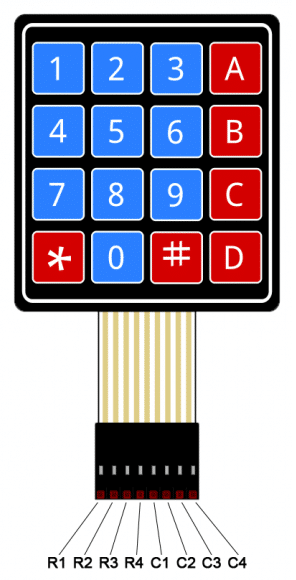
\includegraphics[width=4cm]{images/numpad.png}
  \caption{4$\times$4 numpad} \label{fig:numpad}
\end{figure}


Let op: in de video worden de GPIO-pinnen van je Raspberry Pi als volgt verbonden (zie ook Figuur~\ref{fig:numpad}, en de pinout van de Raspberry pi\footnote{\url{https://pinout.xyz}}.

\section{Aansluiten}

\begin{table}[h]
  \centering
  \begin{tabular}{|r|c|c|}
    \hline
    & \bf Physical RPi pin & \bf BCM \\
    \hline
      \tt R1 & 7 & 4 \\
    \hline
      \tt R2 & 11 & 17 \\
    \hline
      \tt R3 & 13 & 27 \\
    \hline
      \tt R4 & 15 & 22 \\
    \hline
      \tt C1 & 12 & 18 \\
    \hline
      \tt C2 & 16 & 23 \\
    \hline
      \tt C3 & 18 & 24 \\
    \hline
      \tt C4 & 22 & 25 \\
    \hline
  \end{tabular}
  \caption{Aansluiten RC522 op Raspberry Pi}\label{tab:pins}
\end{table}

\end{document}
